\chapter{研究背景}

近些年来,数据量的巨幅增长,尤其是从2005年到2010年,全球产生的数据量增长了10倍(从130艾字节增长到了1227艾字节),目前仍在继续增长\cite{gantz2012digital,villars2011big}。数据交易的市场也以惊人的速度发展着,预计从目前到2020年,大数据和其商业分析的市场规模会从1301亿美元增长到2030亿美元\cite{idc}。如今,高质量和可信赖的数据商品及其相关的分析业务有着巨量的市场需求\cite{gantz2012digital,maitland2002european,turner2014digital,villars2011big}。

\begin{figure}[!htp]
  \centering
  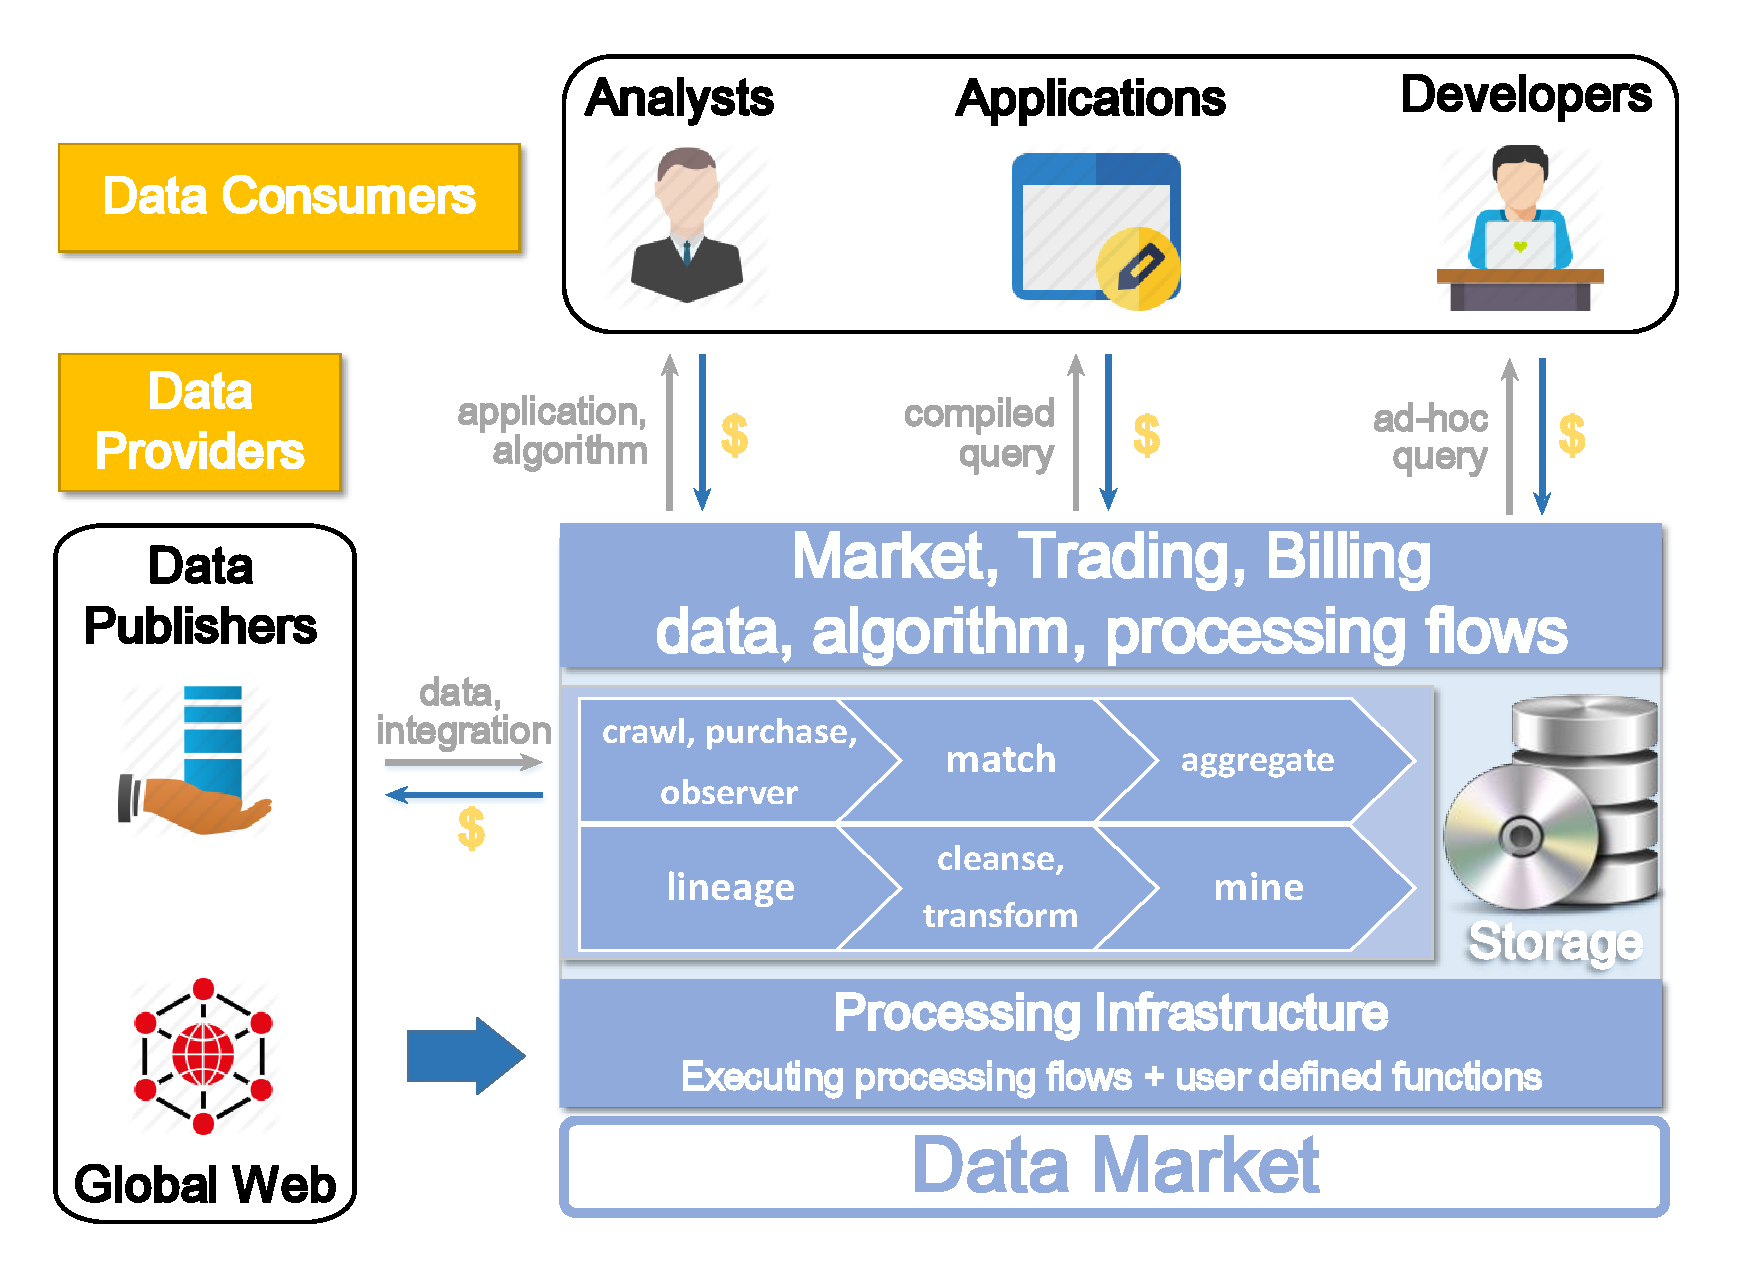
\includegraphics[width=0.65\textwidth]{chapter1/data_market_flow.pdf}
  \bicaption[fig:data market flow]{数据市场数据流动示意图}{数据市场数据流动示意图}{Fig}{Data Flow in Data Market}
\end{figure}

现在,数据商品和相关分析业务主要是由在线数据市场提供的。这些市场从数据发布者和全球网络收集数据,并对其进行清洗、挖掘和整理,然后出售给不同的消费者,如图\ref{fig:data market flow}所示。具体来说,数据消费者主要由开发者和中小企业主构成。这些数据消费者需要在线数据市场提供的数据和相关分析业务来帮助他们做商业决策。至于在线数据市场,他们在整理过的、有价值的数据的基础上,提供分析、商业应用和算法等服务给消费者。现在,国外主要有三家数据交易平台,分别是Microsoft Windows Azure Data Marketplace\cite{MicrosoftAzure}, Inforchimps\cite{infochimps}以及Factual\cite{factual}。而国内也主要有三家平台,分别是贵阳大数据交易所\cite{gbdex},武汉长江大数据交易中心和武汉东湖大数据交易中心\cite{chinadatatrading}。然而,在这些国内外数据交易平台,并没有一个统一的定价机制来指导整个市场。因此,当前数据产品的定价处于一个比较混乱的阶段。不同的数据交易平台采用的是不同的定价机制,而其中最普遍采用的有四种种机制:基于订阅的定价机制、基于查询的定价机制,捆绑销售定价机制以及私下协商定价机制。选择什么样的定价机制具体取决于消费者使用模式以及数据提供商之间的竞争差异。但是,需要指出的是,目前没有任何一种定价机制将数据本身所含有的信息量考虑为定价因素。从消费者角度考虑,目前很多数据消费者通常只对市场上数据集的某些子集感兴趣,他们并不需要购买完整的数据集,而交易平台往往给出的是完整数据集的价格。当消费者购买这些子集时,他们需要知道这些子集所含信息占完整数据集的比例从而评估交易平台给出的子集定价是否合理。从数据交易平台的角度看,如果他们能给出更多的子集数据价格以及它们之间的信息量关系的话,就能给消费者提供一个更加透明的定价关系,从而吸引更多的消费者进行消费。另一方面,目前已有的定价机制并不能产生最大交易剩余,这样会降低买卖双方的交易信心,从而使原本能发生的交易而没有发生,这将会对数据及其相关交易带来极大的经济损失。因此,我们进行了基于信息熵的数据交易的研究课题,期望以数据产品本身的信息量作为定价指标,然后基于这一指标探索更合适的交易机制,从而更好地促进数据交易市场的发展。
